\section{What the joint training needs}
\label{sec:ablations}
Table~\ref{tab:needs} removes one element of Algorithm~\ref{alg:jpc} at a time on Game24 and reads each row against the paragraph of \S\ref{sec:joint} (or \S\ref{sec:pathwise}, \S\ref{sec:jpc_2d}) that introduced the element. The question for every row is the same, whether the run still reaches the reference level and whether it holds it, so the table reports where a run stands early, at its best and at its end; the full checkpoint trajectories are in Appendix~\ref{app:needs_full}. Rows are compared within their block, since the three blocks were run under successive versions of the recipe (Appendix~\ref{app:details}); Figure~\ref{fig:frozen} shows the failure of the first row of block C directly.

\begin{table}[t]
\centering\small
\caption{Ablations of the joint training on Game24, held-out accuracy (\%) at the deployment sampler. \emph{At 500}: the checkpoint after 500 actor iterations; \emph{best}: the highest checkpoint of the run, with its iteration; \emph{final}: the last checkpoint of the schedule (1500 iterations in blocks A and B, 1000 in C). Reference rows are means of three seeds (their \emph{best} is the mean of the per-seed peaks), the other rows single runs; the SFT base is $45.0$. Blocks are compared within themselves: A is Algorithm~\ref{alg:jpc}; B stores five evenly spaced steps of the window in the buffer instead of $k_{\rm hi}$; C is the first version (pooled loss term only, constant learning rate, no AUC check).}
\label{tab:needs}
\resizebox{\linewidth}{!}{%
\begin{tabular}{@{}llccc@{}}
\toprule
tests & variant & at 500 & best (iteration) & final \\
\midrule
\multicolumn{5}{@{}l}{\emph{A. Algorithm~\ref{alg:jpc} (single-step buffer, both loss terms, AUC check, cosine decay)}}\\
 & \hl{reference (3 seeds)} & 56.4 & \textbf{58.8} (750) & 58.0 \\
\S\ref{sec:pathwise}, objective & actor ascends $\mathrm{sig}(V_\phi)$ instead of $V_\phi$ & \ABp{2} & \ABp{7} (500) & \ABp{6} \\
\S\ref{sec:jpc_2d}, pooling & actor ascends $\min_iR_{k,i}$ instead of the mean & \ABm{2} & \ABm{7} (1250) & \ABm{6} \\
 & \emph{Countdown:} reference (3 seeds; base $42.2$) & 46.6 & 50.2 (1250) & 50.0 \\
\S\ref{sec:pathwise}, objective & \emph{Countdown:} actor ascends $\mathrm{sig}(V_\phi)$ & \ABcp{2} & \ABcp{7} (1000) & \ABcp{6} \\
\midrule
\multicolumn{5}{@{}l}{\emph{B. Five-step buffer}}\\
\S\ref{sec:joint}, where the head is refitted & reference (3 seeds) & 57.2 & 58.9 (750) & 58.4 \\
\S\ref{sec:jpc_2d}, supervision & pooled loss term only & 53.2 & 59.0 (1500) & 59.0 \\
\S\ref{sec:joint}, critic ahead of actor & no AUC check & 55.1 & 58.7 (1000) & 57.7 \\
\S\ref{sec:joint}, step size & constant learning rate $10^{-6}$ & 57.7 & 57.9 (750) & 48.7 \\
\S\ref{sec:joint}, step size & learning rate $3\times10^{-6}$ (stopped at 1000) & 48.8 & 58.0 (250) & 30.3 \\
\midrule
\multicolumn{5}{@{}l}{\emph{C. Earlier recipe}}\\
 & reference (3 seeds) & 50.9 & 56.4 (1000) & 56.4 \\
\S\ref{sec:joint}, critic must move & critic frozen after pre-training & 48.0 & 48.4 (250) & \phantom{0}0.3 \\
\S\ref{sec:joint}, critic ahead of actor & $m_{\rm c}{=}1$ head step per actor step & 51.7 & 51.7 (500) & 51.1 \\
 & $m_{\rm c}{=}8$ & 52.3 & 55.2 (1000) & 55.2 \\
\S\ref{sec:joint}, staleness & buffer $N_{\mathcal B}{=}4$k instead of 16k & 50.1 & 56.4 (1000) & 56.4 \\
\S\ref{sec:joint}, one chain & trained under $\gamma4$@16, read at $\gamma56$@64 & 44.3 & 47.0 (1000) & 47.0 \\
 & \quad the same run read at $\gamma4$@16 (base $35.4$) & 38.7 & 42.5 (1000) & 42.5 \\
\bottomrule
\end{tabular}}
\end{table}

\paragraph{The critic must move with the policy.}
The first row of block C is the one that fails outright. Frozen after pre-training, the critic is exploited exactly as~(\ref{eq:biasm}) predicts, and Figure~\ref{fig:frozen} shows the sequence: the update helps for a few hundred iterations, then the critic's value on the training batch is driven towards certainty while the true success of the same batch falls to zero, and the held-out policy follows it down. The remaining rows of the block calibrate how much refitting is enough: two head steps per actor step on the buffer keep the value calibrated, one step falls behind from the middle of the run, eight match two, and a buffer a quarter of the size matches the full one, so within this range the refit is not the bottleneck; \S\ref{sec:exp_critic} shows the case, the pooled head on Countdown, where it becomes one.

\paragraph{What the actor ascends.}
Two rows of block A test the objective. Ascending the critic's probability instead of its log-odds reaches a lower level early and then drifts down, on Game24 and on Countdown alike: the probability's gradient vanishes on the states whose outcome is nearly decided, so the actor's steps concentrate on the remaining ones and the decided states are left to drift, which is why \S\ref{sec:pathwise} ascends the logit. Pooling the field by its minimum instead of its mean costs about three points at every checkpoint: the minimum trains one position per state, the mean trains all of them, the reason \S\ref{sec:jpc_2d} keeps the mean for training and reserves the minimum for ranking single samples.

\paragraph{Where the head is refitted, and the step size.}
Blocks A and B differ in where the buffer's states come from, the top of the window or five steps across it, and on Game24 the two agree within a point; on Countdown, where the outcome is not readable before the middle of the chain, the five-step buffer costs three points (Appendix~\ref{app:needs_full}), which is why Algorithm~\ref{alg:jpc} refits at $k_{\rm hi}$. The second loss term and the AUC check change how fast the first 500 iterations move, not the level reached. The step size is the setting that separates a run that holds from one that collapses, in both blocks: at three times the reference rate the run reaches the reference level in 250 iterations and loses half of it by 1000, at a constant rate it holds for 750 iterations and then loses nine points, and with the cosine decay every seed of Table~\ref{tab:main} holds to its last checkpoint. This is the bias argument of \S\ref{sec:joint}: the error of a refit critic is paid at every actor step in proportion to the step.

\paragraph{One chain.}
The last two rows of block C train under the cheap $\gamma4$@16 chain. The policy improves that chain by seven points and, read at the deployment sampler, ends twelve points below the runs trained there: the value, and with it the improvement, belongs to the chain it was defined on. This is why Algorithm~\ref{alg:jpc} trains under the sampler that will be deployed, and why the loop of \S\ref{sec:loop} is needed to reach the others.

\begin{figure}[t]
\centering
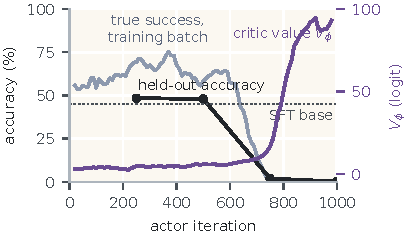
\includegraphics[width=0.9\linewidth]{figures/fig_frozen.pdf}
\caption{Frozen against jointly trained critic on Game24 (2D critic, $10^{-6}$). Red: the critic's value on the training batch; grey: the true success rate of that batch; blue: held-out accuracy at the deployment sampler. With a frozen critic the value is driven towards certainty while success collapses to zero; with the head refitted after every actor step the value stays calibrated and the policy improves.}
\label{fig:frozen}
\end{figure}
